\documentclass{controle}
\usepackage{main}

\title{Baccalauréat général : Épreuve anticipée de mathématiques}
\author{Voie générale : candidats suivant l'enseignement de spécialité de mathématiques}
\date{Durée : 2 heures. L'usage de la calculatrice n'est pas autorisé}

\headrule
\header{Épreuve anticipée de mathématiques}{}{Première Spécialité Mathématiques}
\footer{}{}{Page \thepage{} sur \numpages}

\printanswers
\begin{document}

\begin{coverpages}
\maketitle
\begin{tcolorbox}
\textbf{Indiquez votre nom, prénom et le nom de votre groupe de spécialité sur votre copie.}
\begin{itemize}
\item Groupe 1 : Mr Langlois
\item Groupe 2 : Mr Canu
\item Groupe 3 : Mr Lavigne (Mardi Après-Midi) 
\item Groupe 4 : Mr Lavigne (Mardi Matin)
\item Groupe 5 : Mme Abassi
\end{itemize}
\end{tcolorbox}
\end{coverpages}

\begin{questions}
\titledquestion{Questionnaire à choix multiple}[6]

\hfill
\vspace*{0.25cm}

\textbf{Pour cette première partie, aucune justification n'est demandée et une seule réponse est possible par question. Pour chaque question, reportez son numéro dans votre copie et indiquez votre réponse.}

\vspace*{0.25cm}
\begin{parts}
\part $105$ minutes correspondent à :

\begin{oneparchoices}
\choice $1,05h$
\choice $1,45h$ 
\choice $1,5h$
\correctchoice $1,75h$
\end{oneparchoices}

\vspace*{0.8cm}

\part On considère un nombre réel $x$. Si $x>0$, alors :

\begin{oneparchoices}
\choice $x=x^2$
\choice $x \leq x^2$
\choice $x \geq x^2$
\correctchoice Cela dépend de la valeur de $x$
\end{oneparchoices}

\vspace{0.8cm}

\part On considère la relation : $A=\dfrac{x+6y}{x}$. Lorsque $x=-\dfrac{1}{3}$ et $y=\dfrac{1}{18}$, la valeur de $A$ est : \\

\begin{oneparchoices}
\choice $\dfrac{1}{3}$
\correctchoice $0$
\choice $3$
\choice $-{\dfrac{1}{3}}$
\end{oneparchoices}

\vspace{0.8cm}

\part Le volume d'un cylindre de hauteur $h$ et de rayon $r$ est donné par $V=\pi r^2 h$. On cherche à isoler $h$. On a :

\begin{oneparchoices}
\choice $h=\sqrt{\dfrac{V}{\pi r^2}}$
\choice $h=\dfrac{\pi r^2}{V}$
\correctchoice $h=\dfrac{V}{\pi r^2}$
\choice $h=\dfrac{r^2}{\pi V}$
\end{oneparchoices}

\vspace{0.8cm}

\part Un drapeau a une aire de $3\,m^2$. Cela représente :

\begin{oneparchoices}
\choice $0{,}003\,cm^2$
\choice $0{,}3\,cm^2$
\choice $300\,cm^2$
\correctchoice $30\,000\,cm^2$
\end{oneparchoices}

\vspace{0,8cm}

\part Le prix d'un article est multiplié par $1,11$. Cela signifie que le prix de l'article a subi :

\begin{oneparchoices}
\choice une hausse de $11$ euros
\correctchoice une hausse de $11\%$
\choice une hausse de $1{,}1\%$
\choice une hausse de $111\%$
\end{oneparchoices}

\vspace{0,8cm}

\part Une forme factorisée de l'expression $-3(x+1)+(x+1)^2$ est :

\begin{oneparchoices}
\choice $-(x+1)$
\choice $-(x+1)(x+2)$
\correctchoice $(x+1)(x-2)$
\choice $x^2-x-2$ \\
\end{oneparchoices}

\vspace{0,8cm}

\part Le point qui n'appartient pas à la courbe d'équation $y=\dfrac{6}{x}$ est :

\begin{oneparchoices}
\choice $M(2;3)$
\correctchoice $N(3;3)$
\choice $P(1;6)$
\choice $Q(0,5;12)$
\end{oneparchoices}

\vspace{0,8cm}

\part Une réduction de $50\%$ suivie d'une augmentation de $50\%$ équivaut à :

\begin{oneparchoices}
\choice revenir à la valeur initiale
\correctchoice une baisse de $25\%$
\choice une baisse de $75\%$
\choice une hausse de $75\%$
\end{oneparchoices}

\vspace{0,8cm}

\part Une boite contient 20 billes au total. Dans cette boite, la proportion de billes rouges est égale à 0,3. Le nombre de billes rouges dans la boite est égal à :

\begin{oneparchoices}
\correctchoice $6$
\choice $5$
\choice $3$
\choice $17$
\end{oneparchoices}

\vspace{0,8cm}

\item On peut affirmer que :

\begin{oneparchoices}
  
\correctchoice $\dfrac{12}{13}<\dfrac{13}{14}$
\choice $\dfrac{12}{13}=\dfrac{13}{14}$
\choice $\dfrac{12}{13}>\dfrac{13}{14}$
\choice Il est impossible de comparer ces deux nombres. \\
\end{oneparchoices}

\vspace{0,8cm}

\part La moitié de $10^{24}$ vaut :

\begin{oneparchoices}
\choice $5^{24}$
\choice $10^{12}$
\choice $5^{12}$
\correctchoice $5 \times 10^{23}$ \\
\end{oneparchoices}

\end{parts}

\titledquestion{Fonction exponentielle}[5]

On étudie une fonction $f$ définie sur $[-2;5]$. Sa courbe représentative $\mathcal{C}_f$ est donnée sur le repère ci-dessous :
\begin{center}
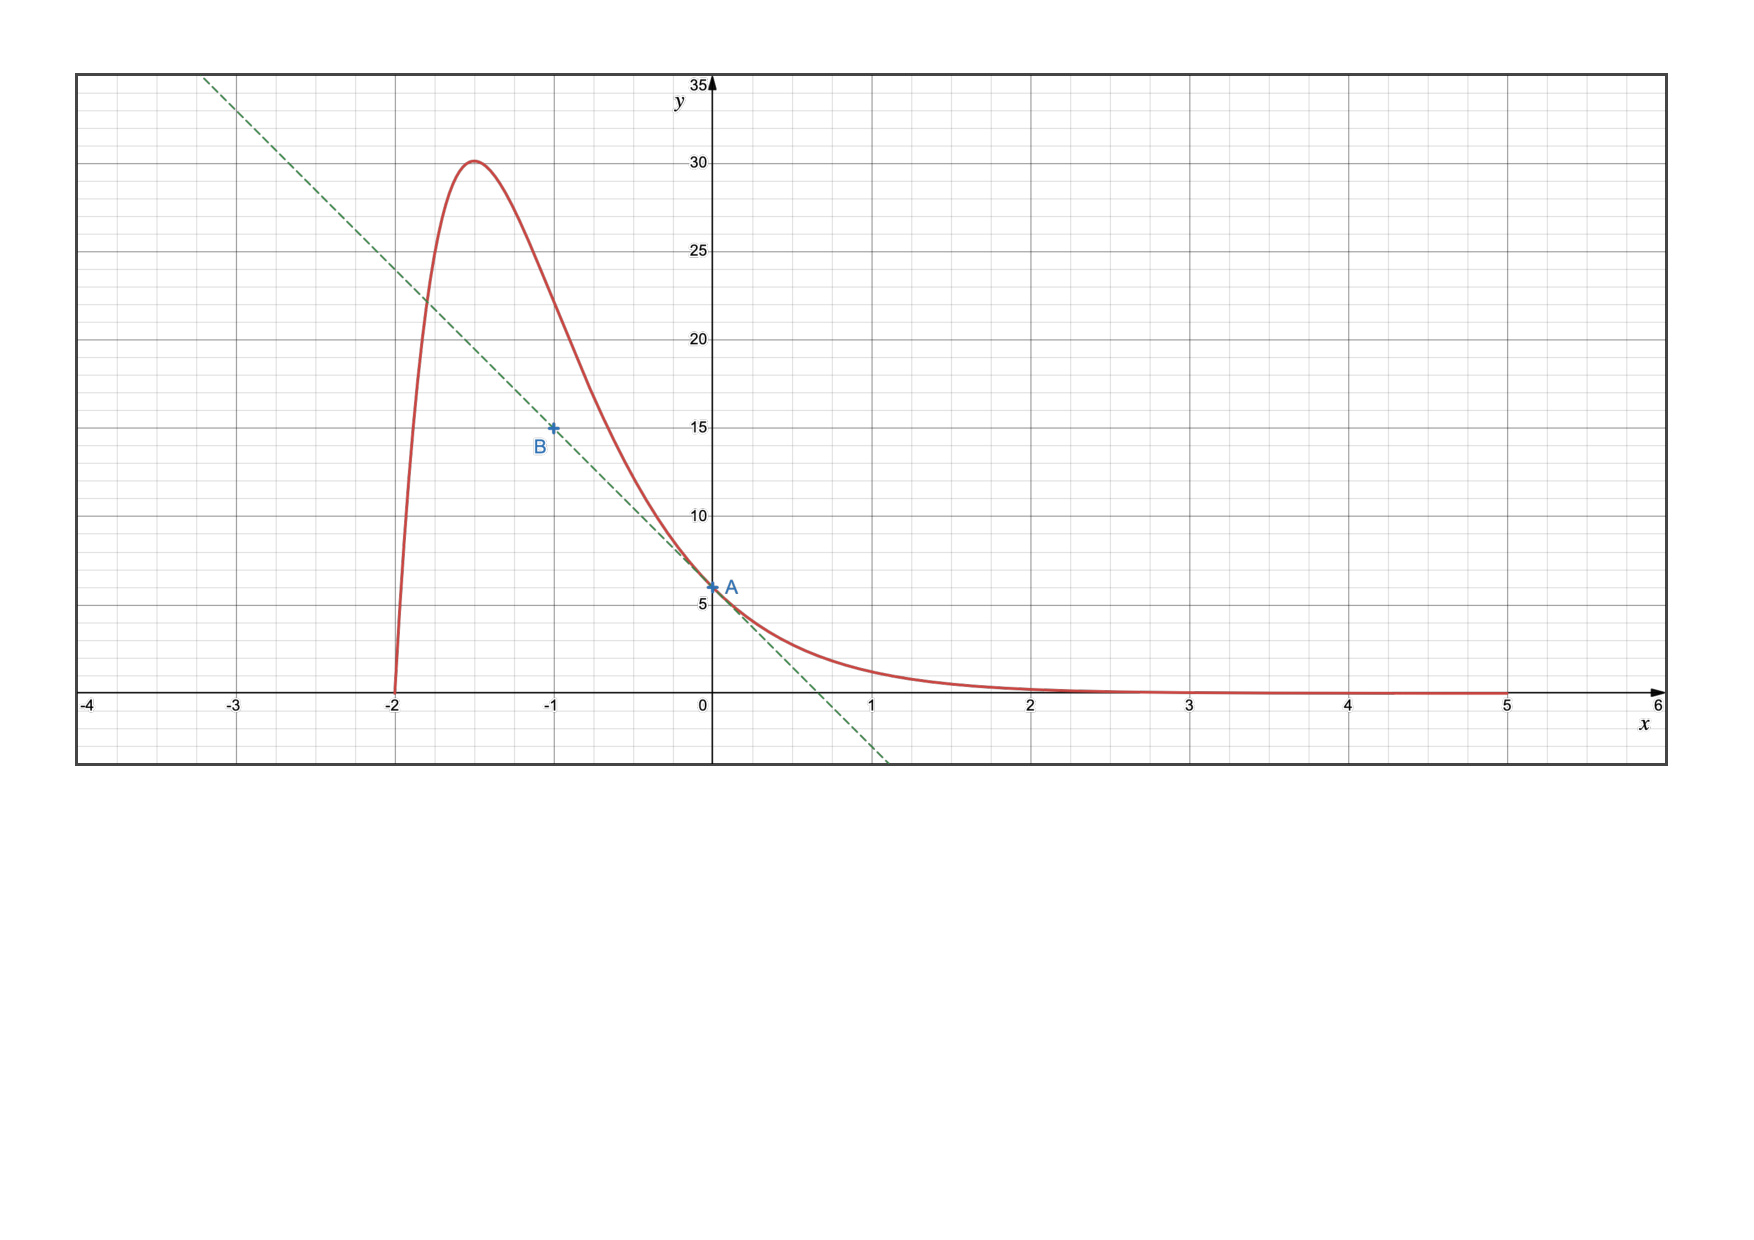
\includegraphics[width=\textwidth,trim={0 7cm 0 1cm}, clip]{Graphique_expo.pdf}
\end{center}
On admet que la fonction est dérivable sur $]-2;5[$. Le point $A(0;f(0))$ appartient à la courbe $\mathcal{C}_f$. On a représenté la droite $(AB)$ qui est la tangente à $\mathcal{C}_f$ en $A$.

\vspace*{0.5cm}

\begin{parts}
\part[0.5] Déterminer graphiquement $f(0)$ et $f'(0)$.
\part[0.5] Résoudre graphiquement, à l'aide de la précision permise par le graphique, l'équation suivante :
\begin{equation*}
f'(x) = 0
\end{equation*}
\part[1] On admet que pour tout $x \in [-2;5]$, on a 
\begin{equation*}
f(x)=(3x+6)e^{-2x}
\end{equation*}
En déduire que $f'(x) = (-6x-9)e^{-2x}$ pour tout $x \in ]-2;5[$.
\part[1] Étudier le signe de $f'$. Justifier votre réponse.
\part[0.5] En déduire le tableau de variations de $f$. On ne demande pas les valeurs des images de $f$ sur le tableau.
\part[0.5] Déterminer par le calcul l'équation de la tangente à $\mathcal{C}_f$ passant par $A(0;f(0))$.
\part[1] En déduire les coordonnées du point d'intersection de $d$ et de l'axe des abscisses.
\end{parts}



\begin{solution}[0.5cm]
\begin{parts}
\part Graphiquement, on obtient $f(0) = 6$ (ordonnée du point $A$). La pente $f'(0)$ de la tangente de la courbe $\mathcal{C}_f$ en $A$ est obtenu en calculant le coefficient directeur de la droite $(AB)$.

\begin{equation*}
f'(0) = \dfrac{y_B - y_A}{x_B - x_A} = \dfrac{15 - 6}{-1 - 0} = -9
\end{equation*}
\part Avoir $x$ solution de $f'(x) = 0$ revient à dire que la tangente à la courbe $\mathcal{C}_f$ est horizontale en le point de coordonnées $(x;f(x))$. Ici, seul $x = -1,5$ semble être solution.
\part La fonction $f$ est dérivable sur $]-2;5[$. La fonction $f$ a pour expression un produit. On donne séparément les dérivées des facteurs du produit.

Soit $g(x) = 3x + 6$ pour tout $x \in ]-2;5[$. Alors $g'(x) = 3$.

Soit $h(x) = e^{-2x}$ pour tout $x \in ]-2;5[$. Alors, pour obtenir la dérivée de $h$, on procède à un changement de variable.

\begin{equation*}
(e^{-2x})' \underset{X = -2x}{=} (e^X)' = X'e^X = (-2x)'e^{-2x} = -2e^{-2x}
\end{equation*}

Ainsi, $h'(x) = -2e^{-2x}$.

On en déduit, par dérivation d'un produit de fonctions dérivables, que
\begin{equation*}
\begin{aligned}
f'(x) &= g'(x)h(x) + g(x)h'(x)\\ 
&= 3e^{-2x} + (3x + 6)(-2e^{-2x})\\ 
&= (3 -2(3x + 6))e^{-2x}\\ 
&= (-6x - 9)e^{-2x}
\end{aligned}
\end{equation*}
\part On trace le tableau de signes de $f'(x)$. Pour cela, on remarque que $e^{-2x} > 0$ pour tout $x \in ]-2;5[$. On en déduit que le signe de $f'(x)$ est uniquement dépendant du signe de $(-6x - 9)$, qui est l'expression d'une fonction affine. Celle-ci s'annule en $-1,5$ et est décroissante.
\begin{center}
\begin{tikzpicture}
\tkzTabInit{$x$ / 1, Signe de $e^{-2x}$ / 1.5, Signe de $(-6x - 9)$ / 1.5, Signe de $f'$ / 1.5}{$-2$, $-1.5$, $5$};
\tkzTabLine{,,+,,};
\tkzTabLine{,+,z,-,};
\tkzTabLine{,+,z,-,};
\end{tikzpicture}
\end{center}
\part On déduit de la réponse précédente le tableau de variations de $f$.
\begin{center}
\begin{tikzpicture}
\tkzTabInit{$x$ / 1, Variations de $f$ / 1.5}{$-2$, $-1.5$, $5$};
\tkzTabVar{-/,+/,-/};
\end{tikzpicture}
\end{center}
\part Par application de la formule du cours,
\begin{equation*}
y = f'(0)(x - 0) + f(0) = -9x + 6
\end{equation*}
\part On cherche donc le point de coordonnées $(x;y)$ satisfaisant l'équation de la tangente $y = -9x + 6$ et l'équation de l'axe des abscisses $y = 0$. On en déduit que $x$ est solution de l'équation $-9x + 6 = 0$.

Ainsi, $x = \dfrac{-6}{-9} = \dfrac{2}{3}$.

Le point d'intersection a pour coordonnées $\left(\dfrac{2}{3};0\right)$.
\end{parts}
\end{solution}




\titledquestion{Suites numériques}[5]
On considère la suite $(u_n)$ définie par récurrence par $u_0 = 5$ et, pour tout $n \in \N$, par
\begin{equation*}
u_{n+1} = \dfrac{2u_n}{3u_n + 2} 
\end{equation*}

Le but de cet exercice est de déterminer une formule explicite de $u_n$, de conjecture l'éventuelle limite de cette suite, puis un indice à partir duquel les valeurs prises par la suite sont inférieures à un certain seuil. 

\vspace*{0.5cm}

\begin{parts}
\part[0.75] Calculer $u_1$, $u_2$ et $u_3$.
\part[1] Déterminer le sens de variation de la suite $(u_n)$. \textbf{On admet que tous les termes $u_n$ sont strictement positifs.}

On pose la suite $(w_n)$ de terme général
\begin{equation*}
w_n = \dfrac{1}{u_n}
\end{equation*}
pour tout $n \in \N$.
\part[0.75] Montrer que pour tout $n \in \N$,
\begin{equation*}
w_{n+1} - w_n = \dfrac{3}{2}
\end{equation*}
\part[0.5] Justifier alors que la suite $(w_n)$ est arithmétique, en précisant son premier terme $w_0$ et sa raison $r$.
\part[0.25] En déduire l'expression de $w_n$ en fonction de $n$.
\part[0.75] Montrer alors que pour tout $n$, on a
\begin{equation*}
u_n = \dfrac{10}{2 + 15n}
\end{equation*}
\part[0.25] En déduire $u_{20}$.
\part[0.25] La suite $u_n$ semble-t-elle admettre une limite ? Si oui, laquelle ? \textbf{On utilisera la table de valeurs ci-dessous.}

\begin{equation*}
\begin{pycode}
def f(n):
  return f"{10.0/(2.0+15.0*n):.3f}"

L = [1,10,50,100,150,200,500]
fL = list(map(f,L))
print(r"\begin{tblr}{hlines,vlines, columns = {mode=dmath}}")
print(r"n &" + " & ".join(list(map(str,L))) + r"\\")
print(r"u_n \simeq &" + " & ".join(list(map(str,fL))) + r"\\")
print(r"\end{tblr}")
\end{pycode}
\end{equation*}
 
\part[0.5] Déterminer le plus petit rang $n$ à partir duquel les termes $u_n$ sont inférieurs à $0.01$.
\end{parts}

\begin{solution}
\begin{parts}
\part 
\begin{itemize}
\item $u_1 = \dfrac{2u_0}{3u_0 + 2} = \dfrac{10}{17}$
\item $u_2 = \dfrac{2u_1}{3u_1 + 2} = \dfrac{\dfrac{20}{17}}{\dfrac{30}{17}+2} = \dfrac{\dfrac{20}{17}}{\dfrac{64}{17}} = \dfrac{20}{17} \times \dfrac{17}{64} = \dfrac{20}{64} = \dfrac{5}{16}$
\item $u_3 = \dfrac{2u_2}{3u_2 + 2} = \dfrac{\dfrac{10}{16}}{\dfrac{15}{16}+2} = \dfrac{\dfrac{10}{16}}{\dfrac{47}{16}} = \dfrac{10}{16} \times \dfrac{16}{47} = \dfrac{10}{47}$
\end{itemize}
\part Pour déterminer le sens de variation de $(u_n)$, on compare $\dfrac{u_{n+1}}{u_n}$ et $1$. En effet, une telle division est possible car $u_n$ est strictement positif (et donc non nul) pour tout $n \in \N$.

Soit $n \in \N$. Alors,
\begin{equation*}
\begin{aligned}
\dfrac{u_{n+1}}{u_n} &= \dfrac{\dfrac{2u_n}{3u_n + 2}}{u_n}\\
&= \dfrac{2\cancel{u_n}}{(3u_n + 2)\cancel{u_n}}\\
&= \dfrac{2}{3u_n + 2}
\end{aligned}
\end{equation*}
Comme $u_n > 0$, on en déduit que $3u_n + 2 > 2$ et donc que cette fraction est toujours strictement inférieure à $1$.

On en conclut que la suite $(u_n)$ est décroissante.

\part Soit $n \in \N$. Alors,
\begin{equation*}
\begin{aligned}
w_{n+1} - w_n &= \dfrac{1}{u_{n+1}} - \dfrac{1}{u_n}\\
&= \dfrac{1}{\dfrac{2u_n}{3u_n + 2}} - \dfrac{1}{u_n}\\
&= \dfrac{3u_n + 2}{2u_n} - \dfrac{1}{u_n}\\
&= \dfrac{3u_n + 2}{2u_n} - \dfrac{2}{2u_n}\\
&= \dfrac{3u_n + 2 - 2}{2_un}\\
&= \dfrac{3\cancel{u_n}}{2\cancel{u_n}}
&= \dfrac{3}{2}
\end{aligned}
\end{equation*}
\part On a pour tout $n \in \N$, $w_{n+1} = w_n + \dfrac{3}{2}$. C'est l'expression par récurrence d'une suite arithmétique de raison $r = \dfrac{3}{2}$. Son premier terme $w_0$ est donné par $w_0 = \dfrac{1}{u_0} = \dfrac{1}{5}$.
\part La suite $(w_n)$ étant arithmétique, on en déduit que sa formule explicite est, pour tout $n \in \N$,
\begin{equation*}
w_n = w_0 + nr = \dfrac{1}{5} + n \dfrac{3}{2} = \dfrac{2 + 15n}{10}
\end{equation*}
\part Soit $n \in \N$. On sait que $u_n = \dfrac{1}{w_n}$. On en déduit que $u_n = \dfrac{1}{\dfrac{2+15n}{10}} = \dfrac{10}{2 + 15n}$. 
\part On calcule $u_{20} = \dfrac{10}{2 + 15 \times 20} = \dfrac{10}{302} = \dfrac{5}{151}$.
\part La suite $(u_n)$ semble admettre $0$ comme limite finie : ses valeurs se \og rapprochent \fg de $0$ au fur et à mesure que $n$ augmente.
\part On cherche $n$ à partir duquel $u_n < \dfrac{1}{100}$. Donc,
\begin{equation*}
\begin{aligned}
u_n < \dfrac{1}{100} &\Leftrightarrow \dfrac{10}{2+15n} < \dfrac{1}{100} \\
&\Leftrightarrow 10 \times 100 < 2 + 15n\\
&\Leftrightarrow 1000 < 2 + 15n\\
&\Leftrightarrow 998 < 15n\\
&\Leftrightarrow \dfrac{998}{15} < n\\
\end{aligned}
\end{equation*}
Puisque $\dfrac{998}{15} \simeq 66,5$, on en déduit que $n = 67$ est la solution recherchée.
\end{parts}
\end{solution}
\newpage




\titledquestion{Probabilités}[4]

Après avoir corrigé les copies du premier bac blanc, le désespoir gagne Madame Abassi. Pour noyer son chagrin et améliorer ses compétences de basketteuse, elle s’entraîne à jeter ses copies dans la boîte qu’avaient confectionné pour elle Messieurs Canu, Langlois et Lavigne.

\vspace*{0.5cm}

Avant de la lancer, elle réalise avec une copie ou bien un avion, ou bien une boulette :
\begin{itemize}
\item On note $A$ l'événement \og Madame Abassi lance un avion \fg{} et on admet que $P(A) = \dfrac{7}{10}$;
\item On note donc $\overbar{A}$ l'événément \og Madame Abassi lance une boulette \fg;
\item On note $R$ l'événement \og Madame Abassi a réussi son tir\fg. 
\end{itemize}

\vspace*{0.5cm}

Après d'inombrables tentatives, l'expérience montre que :
\begin{itemize}
\item Si Madame Abassi lance un avion, la probabilité qu'elle réussisse son tir vaut $\dfrac{1}{10}$ 
\item Si Madame Abassi lance une boulette, la probabilité qu'elle réussisse son tir vaut $\dfrac{6}{10}$ 
\end{itemize}

\vspace*{0.5cm}

Les affirmations suivantes sont-elles vraies ou fausses ? \textbf{Justifier. Tout réponse non justifiée ne rapportera aucun point. Les questions 1 et 2 sont indépendantes.}

\vspace*{0.5cm}
\begin{parts}
\part
\begin{subparts}
\subpart[1] La probabilité que Madame Abassi rate son tir est de $\dfrac{3}{4}$.
\subpart[1] Les événements $A$ et $R$ sont indépendants.
\subpart[1] Sachant qu'elle a réussi son tir, la probabilité que Madame Abassi ait réalisé ce tir avec une boulette vaut $0.72$.
\end{subparts}
\vspace*{0.5cm}

Après des semaines d’entraînement, Madame Abassi gagne en précision. 

Elle joue désormais au basket, et quand elle lance le ballon, la probabilité qu’elle marque un panier vaut $0.5$.

Pour intégrer l’équipe de France de basket, elle passe une épreuve qui consiste à faire trois lancers indépendants : si elle réussit à marquer au moins un panier, Madame Abassi pourra représenter le pays aux Jeux Olympiques de Los Angeles.

\vspace*{0.5cm}

\part[1] La probabilité que Madame Abassi intègre l'équipe de France de basket vaut $\dfrac{7}{8}$.
\end{parts}



\begin{solution}
\begin{parts}
\part 
\begin{subparts}

\subpart On utilise la formule des probabilités totales sur l'événement $\overbar{R}$ avec la partition d'événement $A$ et $\overbar{A}$ (ou on dessine un arbre pondéré de probabilités résumant la situation). Puis on utilise la formule des probabilités composées.

\begin{equation*}
\begin{aligned}
P(\overbar{R}) &= P(\overbar{R} \cap A) + P(\overbar{R} \cap \overbar{A})\\
&= P(A)P_A(\overbar{R}) + P(\overbar{A})P_{\overbar{A}}(\overbar{R})\\
&= \dfrac{7}{10} \times \dfrac{9}{10} + \dfrac{3}{10} \times \dfrac{4}{10}\\
&= \dfrac{63}{100} + \dfrac{12}{100}\\
&= \dfrac{75}{100}\\
&= \dfrac{3}{4}\\
\end{aligned}
\end{equation*}
L'affirmation est donc vraie.
\subpart On constate que $A$ et $\overbar{R}$ ne sont pas indépendants. En effet, $P(\overbar{R}) = \dfrac{3}{4} \neq \dfrac{3}{10} = P_{A}(\overbar{R})$.

On en déduit que $A$ et $R$ ne sont pas indépendants. L'affirmation est donc fausse.
\subpart On cherche à calculer $P_R(\overbar{A})$. Or, $P_R(\overbar{A}) = \dfrac{P(R \cap \overbar{A})}{P(R)}$. On doit donc calculer $P(R \cap \overbar{A})$ et $P(R)$.

On sait grâce à la première affirmation que $P(R) = 1 - \dfrac{3}{4} = \dfrac{1}{4}$. Quant à $P(R \cap \overbar{A})$, on utilise la formule des probabilités composées.

\begin{equation*}
\begin{aligned}
P(R \cap \overbar{A}) = P(\overbar{A})P_{\overbar{A}}(R) = \dfrac{3}{10} \times \dfrac{6}{10} = \dfrac{18}{100}
\end{aligned}
\end{equation*}

Ainsi, $P_R(\overbar{A}) = \dfrac{P(R \cap \overbar{A})}{P(R)} = \dfrac{\dfrac{18}{100}}{\dfrac{1}{4}} = \dfrac{18}{100} \times 4 = \dfrac{18 \times 4}{100} = \dfrac{72}{100} = 0.72$.

L'affirmation est donc vraie.
\end{subparts}

\part On pose les événements de succès de chaque lancer $L_1$, $L_2$ et $L_3$. Ces événements sont indépendants. Plutôt que de calculer directement la probabilités de réussir un de ces lancers, on va calculer la probabilité de rater les trois lancers.

\begin{equation*}
P(L_1 \cap L_2 \cap L_3) = P(\overbar{L_1}) \times P(\overbar{L_2}) \times P(\overbar{L_3}) = \dfrac{1}{2} \times \dfrac{1}{2} \times \dfrac{1}{2} = \dfrac{1}{2^3} = \dfrac{1}{8}
\end{equation*}

Ainsi, la probabilité de réussir au moins un des trois lancers est de $\dfrac{7}{8}$.
\end{parts}
\end{solution}
\end{questions}
\end{document}